\chapter{Introducción}

%No se menciona 'proyeccion sobre superficies irregulares directamente'%

La proyección de imágenes sobre una superficie plana mediante un foco luminoso es una técnica que tiene variadas aplicaciones, siendo de las más utilizadas la proyección de películas cinematográficas. En los últimos tiempos se introdujeron dispositivos de video que permiten proyectar la salida de una computadora, comúnmente utilizados en ámbitos empresariales y académicos, con fines de dictado de cursos y presentaciones. En los últimos años se popularizó la proyección de imágenes y videos sobre fachadas, monumentos u otros objetos tridimensionales de modo de resaltar, ocultar o transformar regiones de interés, técnica que recibe el nombre de \emph{video mapping}.
Un espectáculo de \emph{video mapping} es una expresión artística en la que un \emph{VJ}$^\dagger$\footnote{El símbolo (\dag) representa las referencias al glosario.} presenta su creación mediante la proyección de diversos efectos visuales que generalmente son acompañados por efectos de sonido.
Todo esto se logra mediante la utilización de software especializado, distorsionando las imágenes y videos proyectados.

%Estos espectáculos pueden ser proyecciones sobre fachadas, instalaciones en las cuales se proyecta el espectáculo sobre una superficie irregular como una maqueta en una muestra o una plaza en donde las personas interactúan transitando por el lugar, otro tipo de instalación es la que se realiza con participación de actores o bailarines logrando un espectáculo integrando la expresión corporal con la imagen.%
%A continuación se presentan ejemplos de espectáculos de \emph{video mapping} que muestran distintos efectos logrados mediante ésta técnica.
%Se realizan festivales de video e imagen donde las ciudades resaltan sus arquitecturas realizando espectáculos multitudinarios.

Esta tecnica tiene una gran variedad de aplicaciones que van desde fines artisticos hasta publicitarios. Es muy comun observar proyecciones sobre fachadas para celebrar el aniversario de algun edificio emblematico o durante la realizacion de festivales que se llevan a cabo periodicamente en ciertas cuidades. Ejemplo de esto ultimo es el Festival de Lyon REFERENCIA, llevado a cabo en dicha cuidad, donde los asistentes pueden circular libremente durante el transcurso de los espectaculos, atraccion de interes turitico REDONDEAR. Ademas de estos, se realizan espectaculos de menor tamaño, generalmente realiados en espacios cerrados, y sobre objetos tridimensionales que pueden ser generados especificamene para este proposito como maquetas, o ya existenes como ser automoviles, telefonos moviles, calzados, etc. Una nueva tendencia en el ambiente artistico es la incoropracion de \emph{video mapping} en obras teatrales, en la que se busca la interaccion de los actores con las imagnees proyectadas, pasando éstas a formar parte parte de la obra.

Otros efectos que utilizan la estructura de la fachada consisten en iluminar las distintas secciones de la fachada con distintos colores y produciendo una serie de efectos, ejemplos son las siguientes figuras en las que se utilizan fachadas con infinidad de desniveles iluminando cada sección con un color distinto.
\begin{figure}[H]
  \centering
    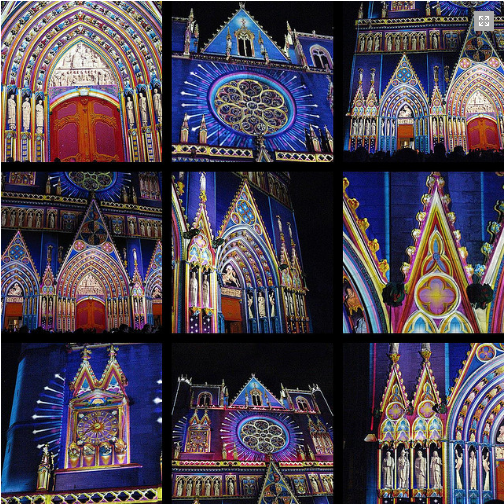
\includegraphics[width=0.5\textwidth]{./Cap1_intro/Fachada1.png}
  \caption[http://www.weltlighting.com/]{Fachada festival Lyon}
  \label{fig:Fachada1}
\end{figure}

En las siguientes imágenes se presenta una instalación sobre una maqueta de caras triangulares construida para el espectáculo, cada cara es iluminada con videos y colores, un efecto muy utilizado es el delineado de los bordes de cada cara.

\begin{minipage}{0.50\textwidth}
\begin{flushleft} \large
\begin{figure}[H]
  \centering
    \includegraphics[width=0.7\textwidth]{./Cap1_intro/Instalacion5.png}
  \caption[http://www.weltlighting.com/fragment/]{Bordes resaltados.}
  \label{fig:Instalacion1}
\end{figure}
\end{flushleft}
\end{minipage}
\begin{minipage}{0.50\textwidth}
\begin{flushright} \large
\begin{figure}[H]
  \centering
    \includegraphics[width=0.75\textwidth]{./Cap1_intro/Instalacion3.png}
  \caption[http://www.weltlighting.com/fragment/]{Sombra degradé en cada cara.}
  \label{fig:Instalacion2}
\end{figure}
\end{flushright}
\end{minipage}

En el siguiente ejemplo se muestra una instalación interactiva hombre-imagen, en la que se realiza una obra de teatro contemporánea con participación de imágenes proyectadas.

\begin{minipage}{0.50\textwidth}
\begin{flushleft} \large
\begin{figure}[H]
  \centering
    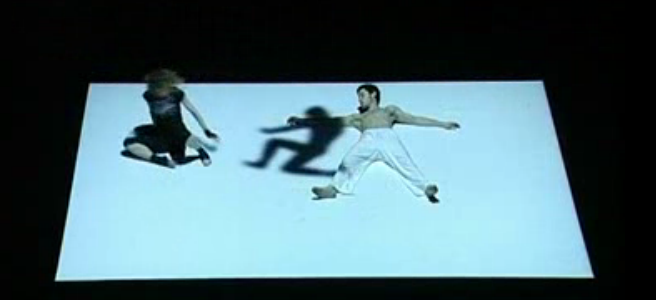
\includegraphics[width=0.7\textwidth]{./Cap1_intro/instalacionHumano1.png}
  \caption[http://vimeo.com/2774865]{Figura humana proyectada.}
  \label{fig:instalacionHumano1}
\end{figure}
\end{flushleft}
\end{minipage}
\begin{minipage}{0.50\textwidth}
\begin{flushright} \large
\begin{figure}[H]
  \centering
    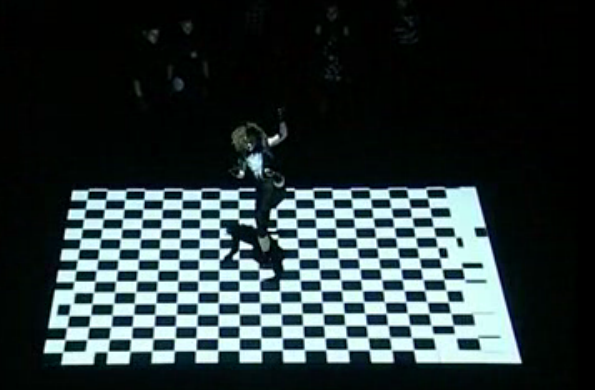
\includegraphics[width=0.75\textwidth]{./Cap1_intro/instalacionHumano4.png}
  \caption[http://vimeo.com/2774865]{Piso damero proyectado.}
  \label{fig:instalacionHumano2}
\end{figure}
\end{flushright}
\end{minipage}

En la figura \ref{fig:Efecto1} y \ref{fig:Efecto2} se presenta un efecto en una herramienta de software realizado con la imagen de la fachada como base realizando distorsiones sobre la misma.

\begin{minipage}{0.50\textwidth}
\begin{flushleft} \large
\begin{figure}[H]
  \centering
    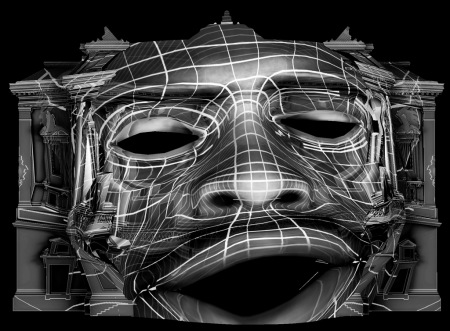
\includegraphics[width=0.7\textwidth]{./Cap1_intro/celestin_head.jpg}
  \caption[http://mappingvideo.blogspot.com/]{Vista del efecto en software.}
  \label{fig:Efecto1}
\end{figure}
\end{flushleft}
\end{minipage}
\begin{minipage}{0.50\textwidth}
\begin{flushright} \large
\begin{figure}[H]
  \centering
    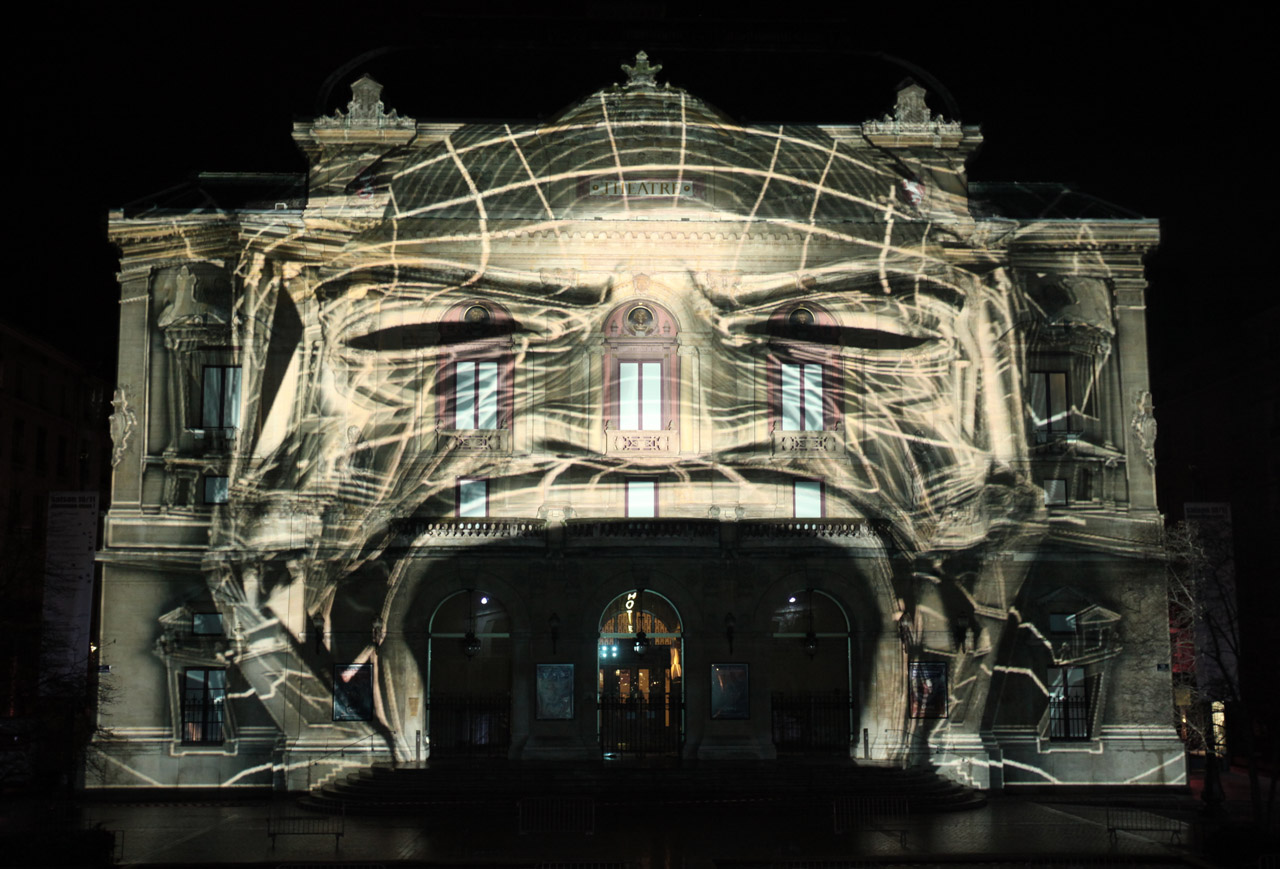
\includegraphics[width=0.75\textwidth]{./Cap1_intro/realcelestins_headshot.jpg}
  \caption[http://mappingvideo.blogspot.com/]{Vista del efecto proyectado.}
  \label{fig:Efecto2}
\end{figure}
\end{flushright}
\end{minipage}

Para la construcción de un espectáculo no existe un proceso definido estándar a seguir sino que cada artista utiliza sus técnicas, métodos y aplicaciones de software de terceros o propias. Aun así se identifican etapas comunes como la construcción de un modelo virtual de la escena, la producción del espectáculo y su proyección. A su vez se identifican dificultades comunes como la calibración de los proyectores al momento de la reproducción y la generación del modelo.

En este proyecto se estudian distintos métodos para facilitar la obtención del modelo virtual. En particular se relevan métodos de escaneo y reconstrucción de objetos tridimensionales y se implementa una de las estrategias estudiadas para su generación.%Ampliar y poner imagenes%
Se desarrolla también una aplicación que permite la creación, edición y reproducción de un espectáculo de \emph{video mapping} basada en un motor tridimensional$^\dagger$. Ésta combina la edición y la reproducción permitiendo visualizar en tiempo real los distintos efectos diseñados. A su vez permite distribuir la reproducción entre varias computadoras, asociadas a uno o más proyectores, y todas sincronizadas por un componente central.
\newpage
%Organización del documento%
Este documento se divide en cuatro capítulos y cuatro apéndices que se describen a continuación.

En el Capítulo 2 - Estado del arte, se explican las nociones básicas de la técnica y las etapas en el proceso de creación que son el modelado, la producción y la calibración. Éstas etapas se presentan mediante dos enfoques: bidimensional y tridimensional. A su vez se explican distintos algoritmos y técnicas para la obtención automática y la reconstrucción de geometría tridimensional.

En el Capítulo 3 - Solución planteada, se presenta la solución propuesta, una herramienta para la edición y posterior ejecución de espectáculos de \emph{video mapping}.

En el Capítulo 4 - Conclusiones y trabajo futuro, se resumen las conclusiones y posibles líneas de trabajo futuro.

Los apéndices extienden los siguientes temas:

En el Apéndice A - Relevamiento de aplicaciones de \emph{video mapping}, se presenta un relevamiento de las aplicaciones existentes más populares utilizadas para la creación de espectáculos.

En el Apéndice B - Aportes, se presentan los resultados de una serie de entrevistas realizadas a \emph{VJs} e ingenieros contactados que contribuyen a la investigación del estado del arte.

En el Apéndice C - Método de triangulación, se detalla el método de triangulación utilizado para la obtención automática de geometría tridimensional.

En el Apéndice D - Modelo de cámara, se explican los fundamentos teóricos del modelo de cámara.


